%% flight-test-analyzer — Technical Proposal
%% Compile with: pdflatex proposal.tex  (run twice for cross-references)

\documentclass[11pt, letterpaper]{article}

\usepackage[margin=1.1in]{geometry}
\usepackage{booktabs}
\usepackage{tabularx}
\usepackage{array}
\usepackage{amsmath}
\usepackage{hyperref}
\usepackage[table]{xcolor}
\usepackage{parskip}
\usepackage{titlesec}
\usepackage{enumitem}
\usepackage{microtype}
\usepackage{caption}
\usepackage{multirow}
\usepackage{appendix}
\usepackage{graphicx}
\usepackage{fancyhdr}
\usepackage{lastpage}
\usepackage{tikz}
\usetikzlibrary{shapes.geometric, arrows.meta, positioning, calc}

\hypersetup{
    colorlinks=true,
    linkcolor=black,
    urlcolor=blue!60!black,
    citecolor=black
}

%% Repo shorthand macros
\newcommand{\repoFTA}{\href{https://github.com/francis-barchesky/flight-test-analyzer}{\texttt{flight-test-analyzer}}}
\newcommand{\repoIADS}{\href{https://github.com/merlinlabs/iads-export}{\texttt{iads-export}}}
\newcommand{\repoTrace}{\href{https://github.com/francis-barchesky/trace-analyzer}{\texttt{trace-analyzer}}}

\titleformat{\section}{\large\bfseries}{}{0em}{}[\titlerule]
\titleformat{\subsection}{\normalsize\bfseries}{}{0em}{}

\newcolumntype{R}[1]{>{\raggedleft\arraybackslash}p{#1}}
\newcolumntype{L}[1]{>{\raggedright\arraybackslash}p{#1}}
\newcolumntype{C}[1]{>{\centering\arraybackslash}p{#1}}

\definecolor{highlight}{RGB}{220, 237, 200}
\definecolor{precursor}{RGB}{255, 243, 205}
\definecolor{context}{RGB}{207, 226, 255}

\pagestyle{fancy}
\fancyhf{}
\renewcommand{\headrulewidth}{0pt}
\fancyfoot[L]{\small Francis Barchesky \quad$\cdot$\quad Merlin Labs}
\fancyfoot[C]{\small Rev.\ 1.0 \quad$\cdot$\quad \today}
\fancyfoot[R]{\small Page \thepage\ of \pageref{LastPage}}

\begin{document}

%% ---------------------------------------------------------------------------
%% Title
%% ---------------------------------------------------------------------------

\begin{center}
  {\LARGE\bfseries Automated Flight Test Failure Analysis} \\[0.5em]
  {\large Model-Aware Upstream Tracing and Fleet-Wide Fault Correlation} \\[1.2em]
  {\normalsize Merlin Labs \quad$\cdot$\quad 208B Flight Test Program} \\[0.3em]
  {\small Francis Barchesky \quad$\cdot$\quad \today \quad$\cdot$\quad Rev.\ 1.0}
\end{center}

\vspace{1em}
\hrule
\vspace{1.5em}

%% ---------------------------------------------------------------------------
%% Abstract
%% ---------------------------------------------------------------------------

\begin{center}
\begin{minipage}{0.88\textwidth}
\small\textit{%
This document describes the \repoFTA{} toolchain: an automated
pipeline for precise, reproducible failure detection and root-cause analysis in
flight test data. The system combines a Simulink model trace graph
(22{,}361 nodes, 137{,}153 edges) with Breadth-First Search upstream traversal
and fleet-wide statistical correlation to distinguish genuine fault precursors
from consequence signals. Applied to 76 sorties and 72 AFCS disengagement
episodes, the toolchain identifies a repeatable precursor sequence with
sub-sample timing precision and completes the 2026 flight testing effort analysis in under
one hour on commodity hardware. This proposal summarises the methodology,
presents initial results, and outlines a path to fully automated continuous
integration within the existing build and data ingestion infrastructure.}
\end{minipage}
\end{center}

\vspace{1.5em}

%% ---------------------------------------------------------------------------
\section*{Executive Summary}
%% ---------------------------------------------------------------------------

\noindent Flight test generates large volumes of IADS time-series data that
currently requires manual, engineer-intensive review to diagnose AFCS
disengagement events. This toolchain replaces that manual process with a
fully automated, reproducible pipeline that runs on every sortie upload.

\medskip
\noindent\textbf{The problem it solves.}\quad
Standard correlation tools cannot separate \emph{cause} from
\emph{consequence} --- signals that drop because a fault already occurred
appear identical to precursor signals. Manual Simulink navigation does not scale
as the model and sortie count grow. Both problems compound when engineers
rotate or are unavailable.

\medskip
\noindent\textbf{How it works.} Three stages run in sequence:
\begin{itemize}[leftmargin=1.6em, itemsep=2pt, topsep=4pt]
  \item \textbf{Build-time (minutes):} \repoTrace{} compiles the Simulink model
    into a 22{,}361-node dependency graph. All cross-model signal paths are
    resolved at build time, not at analysis time.
  \item \textbf{Per-sortie (seconds--minutes):} \repoIADS{} exports raw IADS
    recordings to analysis JSON files. \repoFTA{} processes each sortie
    independently, detecting fault episodes, classifying exit types, and
    computing timing-resolved signal transitions.
  \item \textbf{Fleet-wide (seconds):} Correlation runs across all loaded
    sorties to rank signals by how consistently and how early they change
    before each fault. The upstream BFS trace then filters results to signals
    that are \emph{upstream causes} of the target signal, discarding
    downstream consequences automatically.
\end{itemize}

\medskip
\noindent\textbf{Key results (208B 2026 flight testing, 76 sorties).}
\begin{itemize}[leftmargin=1.6em, itemsep=2pt, topsep=4pt]
  \item 72 AFCS disengagement episodes detected and classified across 34
    affected sorties (45\% fleet exposure).
  \item Response Monitor trips are the leading fault category (42\%),
    concentrated in the takeoff phase --- 18 of 72 events occur in
    T/O\,+\,T/O\,+\,T/O mode.
  \item 24 overtorque events (peak 128.8\% PDI limit) auto-flagged across 8
    sorties, directly linked to the AT-axis Validity Loss cluster (31\% of
    faults).
  \item A three-phase precursor sequence is statistically identified:
    torque context at $-$65 samples, command-path gates at $-$4 to $-$20
    samples, and health/monitor flags at 0--3 samples post-trigger.
  \item Full fleet analysis completes in under one hour on commodity hardware
    using parallel per-sortie workers.
  \item 80 recording gap events detected automatically across 76 sorties;
    causation is currently unknown but gaps have significant testing impact ---
    dropout intervals may mask fault events, truncate pre-trigger analysis
    windows, and suppress mode-state attribution for affected episodes.
\end{itemize}

\medskip
\noindent\textbf{Benefits over manual review.}
\begin{itemize}[leftmargin=1.6em, itemsep=2pt, topsep=4pt]
  \item \textbf{Reproducible:} every sortie is processed by the same logic;
    results do not vary by analyst.
  \item \textbf{Scalable:} analysis time grows sub-linearly; adding sorties
    does not increase per-sortie cost.
  \item \textbf{Cause-filtered:} BFS upstream traversal eliminates the false
    positive burden of consequence signals before an engineer sees results.
  \item \textbf{Integrated:} designed to trigger automatically on IADS upload
    and model build events via existing CI/CD runners (see Section~5).
  \item \textbf{Interactive:} a self-contained HTML viewer requires no
    installation and runs entirely in the browser, enabling immediate
    review in the field.
\end{itemize}

\vspace{0.8em}
\hrule
\vspace{1.5em}

%% ---------------------------------------------------------------------------
\section{Problem Statement}
%% ---------------------------------------------------------------------------

Automatic Flight Control System (AFCS) disengagement events are a recurrent
and high-priority anomaly class during flight test. Diagnosing their root cause
has historically required a skilled engineer to manually step through Simulink
model hierarchies and correlate time-series traces from raw IADS exports --- a
process that is time-consuming, operator-dependent, and difficult to repeat
consistently across a growing fleet dataset.

Two structural weaknesses compound this difficulty. First, standard
signal-correlation tools cannot distinguish a \emph{cause} from a
\emph{consequence}: any signal correlated with a fault transition, including the
many engagement and capability state signals that drop false \emph{because} the
fault occurred, will appear as a top candidate. Second, manual Simulink
navigation does not scale: as the model grows and the sortie count increases,
the space of possible contributing signals expands faster than human review
time.

The \repoFTA{} toolchain addresses both weaknesses directly.

%% ---------------------------------------------------------------------------
\section{Current Process}
%% ---------------------------------------------------------------------------

When an AFCS disengagement event occurs today, the investigation follows a
largely manual sequence. Figure~\ref{fig:current-workflow} illustrates the
end-to-end workflow; the steps below describe each stage in detail.
With 76 sorties in the 2026 flight testing dataset, this process must be
repeated for each affected flight.

\begin{figure}[htbp]
\centering
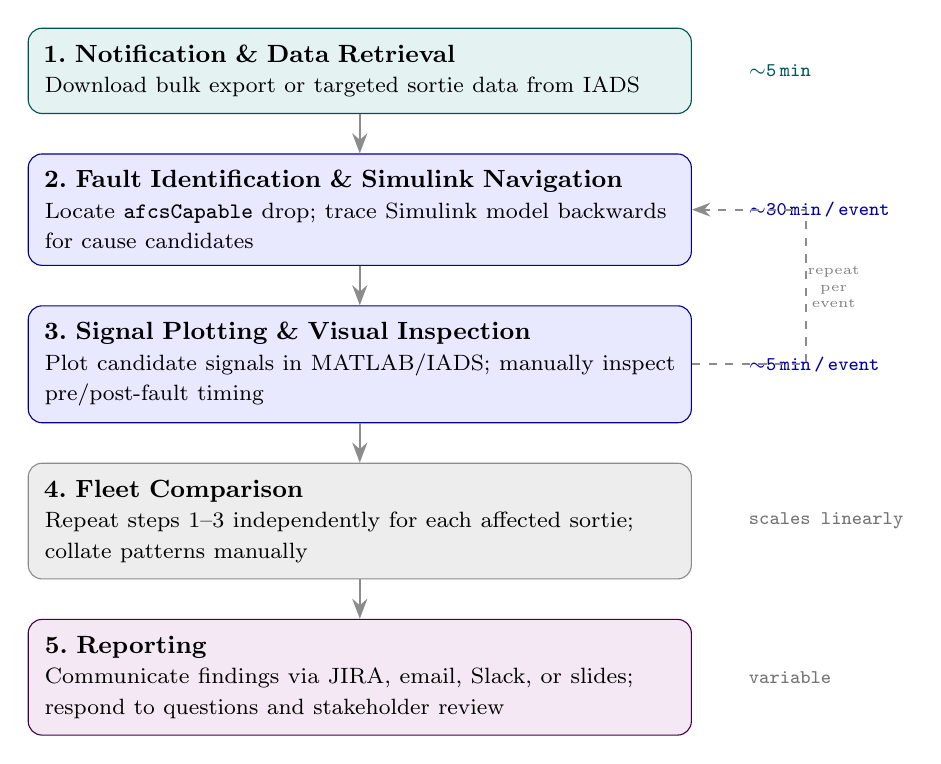
\begin{tikzpicture}[
  node distance   = 0.5cm,
  toolIADS/.style     = {rectangle, rounded corners=5pt,
                          minimum width=8.2cm, minimum height=1.0cm,
                          text width=8.0cm, align=left, font=\small,
                          draw=teal!65!black, fill=teal!10!white, inner sep=6pt},
  toolSIMULINK/.style = {rectangle, rounded corners=5pt,
                          minimum width=8.2cm, minimum height=1.0cm,
                          text width=8.0cm, align=left, font=\small,
                          draw=blue!60!black, fill=blue!9!white, inner sep=6pt},
  toolMANUAL/.style   = {rectangle, rounded corners=5pt,
                          minimum width=8.2cm, minimum height=1.0cm,
                          text width=8.0cm, align=left, font=\small,
                          draw=black!45, fill=black!7, inner sep=6pt},
  toolJIRA/.style     = {rectangle, rounded corners=5pt,
                          minimum width=8.2cm, minimum height=1.0cm,
                          text width=8.0cm, align=left, font=\small,
                          draw=violet!55!black, fill=violet!9!white, inner sep=6pt},
  badge/.style        = {font=\scriptsize\ttfamily, color=#1, align=left},
  arr/.style          = {-{Stealth[scale=1.1]}, thick, color=black!45},
  looparr/.style      = {-{Stealth[scale=1.0]}, thick, dashed, color=black!45, line width=0.8pt},
]

\node[toolIADS] (s1)
  {\textbf{1.\ Notification \& Data Retrieval}\\
   {\footnotesize Download bulk export or targeted sortie data from IADS}};

\node[toolSIMULINK, below=of s1] (s2)
  {\textbf{2.\ Fault Identification \& Simulink Navigation}\\
   {\footnotesize Locate \texttt{afcsCapable} drop; trace Simulink model backwards for cause candidates}};

\node[toolSIMULINK, below=of s2] (s3)
  {\textbf{3.\ Signal Plotting \& Visual Inspection}\\
   {\footnotesize Plot candidate signals in MATLAB/IADS; manually inspect pre/post-fault timing}};

\node[toolMANUAL, below=of s3] (s4)
  {\textbf{4.\ Fleet Comparison}\\
   {\footnotesize Repeat steps 1--3 independently for each affected sortie; collate patterns manually}};

\node[toolJIRA, below=of s4] (s5)
  {\textbf{5.\ Reporting}\\
   {\footnotesize Communicate findings via JIRA, email, Slack, or slides; respond to questions and stakeholder review}};

%% Connecting arrows
\foreach \a/\b in {s1/s2, s2/s3, s3/s4, s4/s5}
  \draw[arr] (\a) -- (\b);

%% Time badges
\node[badge=teal!70!black,  right=0.6cm of s1] {$\sim$5\,min};
\node[badge=blue!65!black,  right=0.6cm of s2] {$\sim$30\,min\,/\,event};
\node[badge=blue!65!black,  right=0.6cm of s3] {$\sim$5\,min\,/\,event};
\node[badge=black!55,       right=0.6cm of s4] {scales linearly};
\node[badge=black!55,       right=0.6cm of s5] {variable};

%% "Repeat per event" loop arrow
\coordinate (rA) at ($(s2.east)+(1.45, 0)$);
\coordinate (rB) at ($(s3.east)+(1.45, 0)$);
\draw[looparr] (s3.east) -- (rB) -- (rA) -- (s2.east);
\node[font=\tiny, color=black!50, align=center]
  at ($(rA)!0.5!(rB)+(0.35,0)$) {repeat\\per\\event};

\end{tikzpicture}
\par\vspace{3pt}
\begin{center}{\setlength{\fboxrule}{0.7pt}\setlength{\fboxsep}{2pt}\tiny\sffamily
\fcolorbox{teal!65!black}{teal!10!white}{\rule{0pt}{5pt}\hspace{8pt}}\;IADS\quad
\fcolorbox{blue!60!black}{blue!9!white}{\rule{0pt}{5pt}\hspace{8pt}}\;MATLAB\,/\,Simulink\quad
\fcolorbox{black!45}{black!7}{\rule{0pt}{5pt}\hspace{8pt}}\;Manual\quad
\fcolorbox{violet!55!black}{violet!9!white}{\rule{0pt}{5pt}\hspace{8pt}}\;JIRA\,/\,Slack\,/\,Email%
}\end{center}
\caption{Current manual AFCS fault investigation workflow (single sortie).
  Box colour indicates the primary tool required at each step (see legend).
  Steps 2--3 scale with the number of disengagement events per flight.}
\label{fig:current-workflow}
\end{figure}

\subsection*{Tools Required (Current Process)}

\begin{itemize}[leftmargin=1.6em, itemsep=3pt, topsep=4pt]
  \item \textbf{MATLAB / Simulink} --- required for opening the flight control
    model, navigating subsystem hierarchies, tracing signal dependencies, and
    generating time-series plots of candidate signals. Requires a licensed
    installation on the engineer's machine with the correct model version
    checked out.
  \item \textbf{IADS ground station / viewer} --- used to locate fault
    timestamps, inspect raw signal data, and export recordings. Access depends
    on network connectivity to the ground station or availability of bulk
    export archives.
  \item \textbf{Plotting tools} --- signal visualisation requires MATLAB,
    a user-maintained Python/script-based plotting workflow, or manual
    inspection in the IADS viewer. There is no standardised plot format across
    engineers.
  \item \textbf{JIRA / email / Slack / slides} --- findings are communicated
    through unstructured channels (JIRA tickets, email threads, Slack messages,
    and slide decks); no machine-readable output is produced for downstream
    re-use.
\end{itemize}

\medskip
\noindent\textbf{How the toolchain changes the tool requirements.}\quad
The \repoFTA{} HTML viewer provides a browser-native inspection interface that
replicates the key functions of Simulink model navigation without requiring a
MATLAB licence or a local model checkout --- signal upstream traces, mode
state timelines, and fault episode classification are all computed from the
compiled trace graph and displayed interactively in the browser. Plotting of
raw time-series signals (servo torque, AGL, deviation) is embedded in the
viewer for signals captured as \texttt{--plot-signals} during analysis.
Custom or exploratory plots beyond the pre-configured set still require MATLAB
or a user-defined script; this remains the primary tool dependency for
engineers who need ad-hoc signal visualisation.

\medskip

\begin{enumerate}[leftmargin=2em, itemsep=5pt, topsep=6pt]

  \item \textbf{Notification and data retrieval.}
    The engineer learns of an AFCS event through pilot debrief notes or a
    post-flight anomaly report. Investigation requires either a manual
    targeted export of the relevant sortie or, at minimum, the download and
    extraction of one or more bulk exports for local data processing.
    Depending on data availability, export scope, and download time, this
    step takes \textbf{$\sim$5\,min}.

  \item \textbf{Fault identification and Simulink model navigation.}
    The engineer opens the raw IADS export to locate the \texttt{afcsCapable}
    transition and establish the fault timestamp, then opens the Simulink model
    in MATLAB (correct build version required) to trace backwards through
    subsystem hierarchies and identify candidate cause signals. These two
    activities are performed together as a single investigation session: there
    is no automated episode detection, exit-type classification, or model
    traversal --- both require hands-on engineer effort and direct Simulink
    access. This step does not produce a repeatable artifact and requires
    familiarity with the model architecture.
    Time: \textbf{$\sim$30\,min per event}; longer for engineers new to the model.

  \item \textbf{Signal plotting and visual inspection.}
    Candidate signals identified in Step~3 are plotted in IADS viewer or
    MATLAB. The engineer visually inspects which signals changed \emph{before}
    vs.\ \emph{after} the fault --- there is no statistical ranking, no
    automatic timing measurement, and no filter separating causes from
    consequences. Each candidate requires a separate plot. Time:
    \textbf{$\sim$5\,min per event}.

  \item \textbf{Fleet comparison.}
    Steps 1--3 are repeated independently for each affected sortie. Patterns
    across sorties (e.g.\ the same precursor appearing in every event) are
    identified by the engineer from memory or manual notes --- there is no
    automated cross-sortie correlation. Time scales \textbf{linearly} with
    the number of sorties.

  \item \textbf{Reporting.}
    Structured reporting is automated by the toolchain; however, reviewing
    and communicating results --- responding to questions, clarifying findings,
    and discussing implications with the wider team --- may consume additional
    time depending on the complexity of the event and stakeholder engagement.
    Time: \textbf{variable}.

\end{enumerate}

\medskip
\noindent\textbf{Estimated total cost per fault investigation:} $\sim$40\,min
per affected sortie for single-event flights, scaling proportionally for
sorties with multiple events. The 2026 208B dataset provides a concrete
basis for this estimate: \textbf{72 disengagement events} were recorded
across \textbf{34 affected sorties} out of 76 total (45\% fleet exposure).
The per-sortie event count ranges from 1 to 8, with an average of 2.1 events
per affected sortie --- 18 sorties experienced a single event, while the
remaining 16 ranged from 2 to 8 events per flight.

Applying the per-step time estimates above (fault identification, Simulink
navigation, and signal plotting all per event):

\medskip
\begin{center}
\begin{tabular}{@{} r r r r @{}}
\toprule
\textbf{Events / sortie} & \textbf{Sorties} & \multicolumn{2}{c}{\textbf{Est.\ time}} \\
\midrule
1 & 18 & \multicolumn{2}{c}{$\sim$40\,min} \\
2 &  8 & \multicolumn{2}{c}{$\sim$75\,min} \\
3 &  3 & \multicolumn{2}{c}{$\sim$110\,min} \\
4 &  1 & \multicolumn{2}{c}{$\sim$145\,min} \\
5 &  2 & \multicolumn{2}{c}{$\sim$180\,min} \\
7 &  1 & \multicolumn{2}{c}{$\sim$250\,min} \\
8 &  1 & \multicolumn{2}{c}{$\sim$285\,min} \\
\midrule
\textbf{Fleet total} & \textbf{34} & \multicolumn{2}{c}{\textbf{$\sim$45\,h}} \\
\bottomrule
\end{tabular}
\end{center}

\medskip
\noindent The automated toolchain processes all 76 sorties in under one hour
of unattended computation, reducing the investigation burden to the time
required to review and act on the generated report.

\subsection*{Proposed Automated Workflow}

Figure~\ref{fig:proposed-workflow} shows the automated pipeline that replaces
the manual sequence. Except for the final review step, all stages are
triggered programmatically and require no engineer interaction.

\begin{figure}[htbp]
\centering
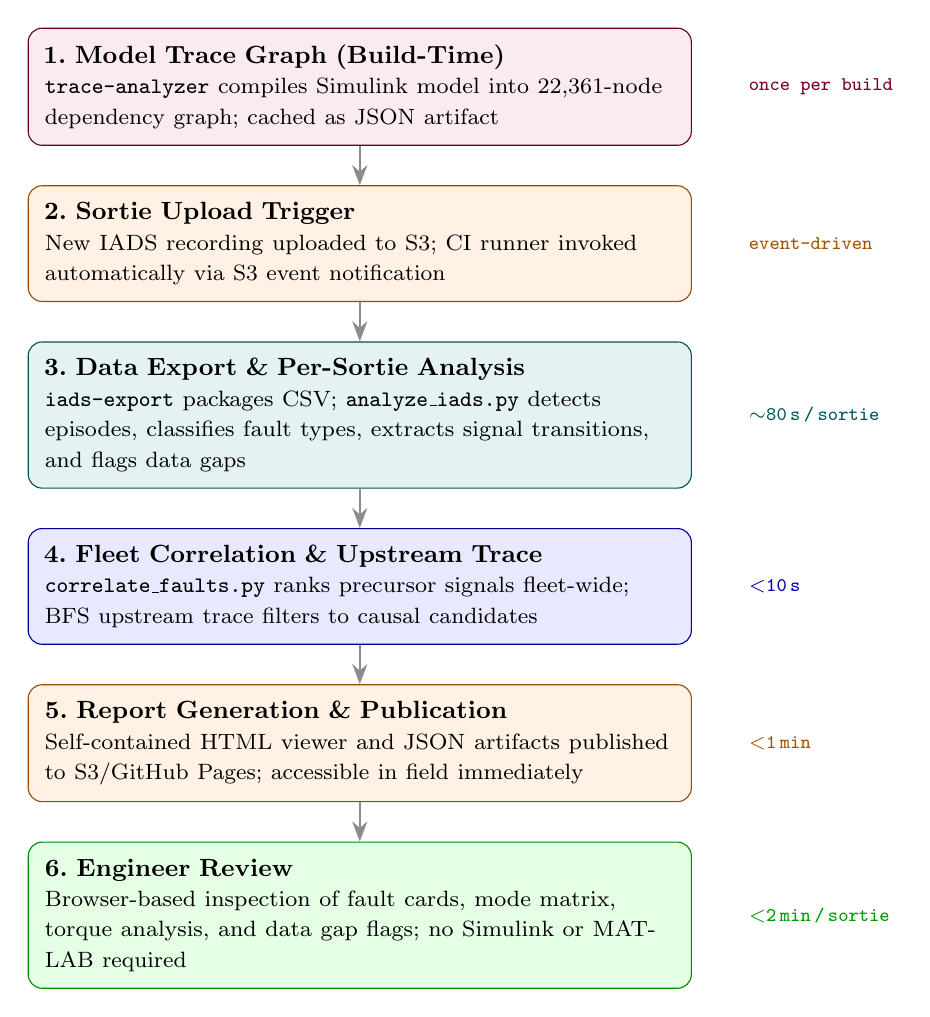
\begin{tikzpicture}[
  node distance   = 0.5cm,
  toolBUILD/.style  = {rectangle, rounded corners=5pt,
                        minimum width=8.2cm, minimum height=1.0cm,
                        text width=8.0cm, align=left, font=\small,
                        draw=purple!55!black, fill=purple!8!white, inner sep=6pt},
  toolCLOUD/.style  = {rectangle, rounded corners=5pt,
                        minimum width=8.2cm, minimum height=1.0cm,
                        text width=8.0cm, align=left, font=\small,
                        draw=orange!60!black, fill=orange!10!white, inner sep=6pt},
  toolIADS/.style   = {rectangle, rounded corners=5pt,
                        minimum width=8.2cm, minimum height=1.0cm,
                        text width=8.0cm, align=left, font=\small,
                        draw=teal!65!black, fill=teal!10!white, inner sep=6pt},
  toolFTA/.style    = {rectangle, rounded corners=5pt,
                        minimum width=8.2cm, minimum height=1.0cm,
                        text width=8.0cm, align=left, font=\small,
                        draw=blue!60!black, fill=blue!9!white, inner sep=6pt},
  toolENG/.style    = {rectangle, rounded corners=5pt,
                        minimum width=8.2cm, minimum height=1.0cm,
                        text width=8.0cm, align=left, font=\small,
                        draw=green!55!black, fill=green!10!white, inner sep=6pt},
  badge/.style      = {font=\scriptsize\ttfamily, color=#1, align=left},
  arr/.style        = {-{Stealth[scale=1.1]}, thick, color=black!45},
]

\node[toolBUILD] (p1)
  {\textbf{1.\ Model Trace Graph (Build-Time)}\\
   {\footnotesize \texttt{trace-analyzer} compiles Simulink model into 22{,}361-node dependency graph; cached as JSON artifact}};

\node[toolCLOUD, below=of p1] (p2)
  {\textbf{2.\ Sortie Upload Trigger}\\
   {\footnotesize New IADS recording uploaded to S3; CI runner invoked automatically via S3 event notification}};

\node[toolIADS, below=of p2] (p3)
  {\textbf{3.\ Data Export \& Per-Sortie Analysis}\\
   {\footnotesize \texttt{iads-export} packages CSV; \texttt{analyze\_iads.py} detects episodes, classifies fault types, extracts signal transitions, and flags data gaps}};

\node[toolFTA, below=of p3] (p4)
  {\textbf{4.\ Fleet Correlation \& Upstream Trace}\\
   {\footnotesize \texttt{correlate\_faults.py} ranks precursor signals fleet-wide; BFS upstream trace filters to causal candidates}};

\node[toolCLOUD, below=of p4] (p5)
  {\textbf{5.\ Report Generation \& Publication}\\
   {\footnotesize Self-contained HTML viewer and JSON artifacts published to S3/GitHub Pages; accessible in field immediately}};

\node[toolENG, below=of p5] (p6)
  {\textbf{6.\ Engineer Review}\\
   {\footnotesize Browser-based inspection of fault cards, mode matrix, torque analysis, and data gap flags; no Simulink or MATLAB required}};

%% Connecting arrows
\foreach \a/\b in {p1/p2, p2/p3, p3/p4, p4/p5, p5/p6}
  \draw[arr] (\a) -- (\b);

%% Time badges
\node[badge=purple!65!black, right=0.6cm of p1] {once per build};
\node[badge=orange!65!black, right=0.6cm of p2] {event-driven};
\node[badge=teal!70!black,   right=0.6cm of p3] {$\sim$80\,s\,/\,sortie};
\node[badge=blue!65!black,   right=0.6cm of p4] {$<$10\,s};
\node[badge=orange!65!black, right=0.6cm of p5] {$<$1\,min};
\node[badge=green!60!black,  right=0.6cm of p6] {$<$2\,min\,/\,sortie};

\end{tikzpicture}
\par\vspace{3pt}
\begin{center}{\setlength{\fboxrule}{0.7pt}\setlength{\fboxsep}{2pt}\tiny\sffamily
\fcolorbox{purple!55!black}{purple!8!white}{\rule{0pt}{5pt}\hspace{8pt}}\;trace-analyzer\quad
\fcolorbox{orange!60!black}{orange!10!white}{\rule{0pt}{5pt}\hspace{8pt}}\;AWS\,S3\,/\,GitHub\,CI\quad
\fcolorbox{teal!65!black}{teal!10!white}{\rule{0pt}{5pt}\hspace{8pt}}\;iads-export\quad
\fcolorbox{blue!60!black}{blue!9!white}{\rule{0pt}{5pt}\hspace{8pt}}\;flight-test-analyzer\quad
\fcolorbox{green!55!black}{green!10!white}{\rule{0pt}{5pt}\hspace{8pt}}\;Engineer\,/\,Browser%
}\end{center}
\caption{Proposed automated AFCS fault analysis pipeline.
  Box colour indicates the primary tool at each step (see legend).
  All steps except the final engineer review are triggered programmatically.
  Note: teal (\textit{iads-export}) mirrors the IADS tool in Figure~\ref{fig:current-workflow},
  showing that the data source is the same --- only the access method changes.}
\label{fig:proposed-workflow}
\end{figure}

\medskip
\begin{table}[h]
\centering
\caption{Manual process vs.\ automated toolchain.}
\begin{tabularx}{\textwidth}{@{} l X X @{}}
\toprule
\textbf{Aspect} & \textbf{Current (Manual)} & \textbf{Automated (\repoFTA{})} \\
\midrule
Time to first result    & $\sim$40\,min per sortie (1 event) & $<$\,2\,min per sortie \\
Fleet-wide view         & Sorties reviewed in isolation     & All sorties simultaneously \\
Cause vs.\ consequence  & Engineer judgment                 & Structural (BFS trace graph) \\
Reproducibility         & Engineer-dependent                & Deterministic \\
Overtorque detection    & Separate manual review            & Automatic per sortie \\
Model knowledge at review & Deep Simulink expertise required & None \\
Scales with sortie count & Linearly (hours)                 & Sub-linearly (seconds) \\
Trigger                 & Ad-hoc, after engineer availability & Automatic on IADS upload \\
Output format           & Unstructured (email / slides)     & Structured JSON + HTML report \\
\bottomrule
\end{tabularx}
\end{table}

%% ---------------------------------------------------------------------------
\section{Technical Approach}
%% ---------------------------------------------------------------------------

\subsection{Model Trace Graph}

The foundation of the analysis is a compiled signal-dependency graph derived
from the Simulink flight control model, produced by the \repoTrace{} tool
(\texttt{traceData-EOC-714-00001-05.01.02.json}). This graph contains
\textbf{22{,}361 nodes} and \textbf{137{,}153 directed edges}, where each node
represents a signal port (block output, Inport, Outport, or TestPoint) and each
edge represents a computational dependency from one signal to another.

Unlike documentation or manually maintained dependency matrices, the trace graph
is generated directly from the model and therefore reflects the \emph{actual}
software architecture at a specific build version. Signal paths that cross model
reference boundaries --- for example, the path from a subsystem health monitor
inside \texttt{ApCapable} into the AFCS capability AND gate inside
\texttt{AfcsCapable} --- are fully represented.

\subsection{Breadth-First Search Upstream Traversal}

Given a target failure signal (e.g.\ \texttt{afcsCapable}), the \repoFTA{}
toolchain locates the signal's output computation node in the trace graph and
initiates a Breadth-First Search (BFS) traversal in the \emph{upstream}
direction --- that is, following edges only toward signals that feed into the
target, never toward signals it drives. This directional constraint is
fundamental: it ensures that every discovered signal is structurally capable of
contributing to the fault, not merely correlated with it.

Dead-end traversal at model boundaries is resolved in priority order:
\begin{enumerate}[itemsep=2pt]
  \item \textbf{Cross-model jump} --- if a subsystem named after the boundary
    signal exists in the graph (e.g.\ \texttt{apCapable} $\to$ subsystem
    \texttt{ApCapable}), the BFS crosses into that subsystem's computation output
    gate. This correctly handles the case where a signal is \emph{received} by
    the current subsystem but \emph{computed} elsewhere.
  \item \textbf{Intra-model logic subsystem} --- for signals computed locally
    within the current model, the BFS searches for a subsystem named
    \texttt{\{signal\}Logic} and enters at its output gate.
  \item \textbf{Generic blockName fallback} --- any node sharing the same block
    name with incoming edges, used only when neither above strategy applies.
\end{enumerate}

Applied to \texttt{afcsCapable} with a maximum depth of 15 hops, the traversal
discovers \textbf{1{,}323 upstream TestPoint signals} spanning the full
dependency cone of the AFCS capability logic.

\subsection{Fleet-Wide Fault Correlation}

For each fault episode, the \repoFTA{} toolchain extracts all signal transitions
occurring in a configurable window around the fault trigger (default: $-5$\,s to
$+1$\,s). Raw IADS data is exported via the \repoIADS{} pipeline, which handles
S3 download, bulk CSV export, and sortie packaging. Across all episodes and
sorties, each signal is characterised by:

\[
  \text{score} = \underbrace{f}_{\text{frequency}}
    \times \underbrace{e^{-|\bar{\Delta t}|/2}}_{\text{proximity}}
    \times \underbrace{e^{-\sigma_{\Delta t}/2}}_{\text{consistency}}
\]

where $f$ is the fraction of episodes in which the signal transitioned,
$\bar{\Delta t}$ is the mean lead/lag relative to the trigger in seconds, and
$\sigma_{\Delta t}$ is the standard deviation of the timing. A signal must
excel on all three dimensions simultaneously to rank highly, making the score
resistant to sporadic noise, single-sortie anomalies, and imprecisely timed
transitions.

Signal normalisation collapses lane-redundant names (FCC1A vs FCC1B) to a
single canonical key, and a configurable exclusion list removes known-consequence
signals --- engagement state flags, capability state signals, and monitor trip
outputs that go false \emph{because of} the fault --- to ensure the output
reflects genuine preconditions.

%% ---------------------------------------------------------------------------
\clearpage
\section{Computational Performance}
%% ---------------------------------------------------------------------------

All analyses run on commodity workstation hardware with no specialised
acceleration. Table~\ref{tab:perf} summarises measured wall-clock times.

\begin{table}[h]
\centering
\caption{Measured computation times across the 208B 2026 flight testing dataset.}
\label{tab:perf}
\begin{tabularx}{\textwidth}{@{}l r X@{}}
\toprule
\textbf{Operation} & \textbf{Time} & \textbf{Notes} \\
\midrule
Load trace graph + build indexes  & $< 5$\,s       & 22{,}361 nodes, 137{,}153 edges (\repoTrace{}) \\
BFS upstream traversal            & $< 2$\,s       & 1{,}323 signals, 15-hop depth (\repoFTA{}) \\
Fault correlation (76 sorties)    & $< 10$\,s      & Reads cached analysis JSONs (\repoFTA{}) \\
\midrule
Per-sortie analysis JSON (median) & $\sim\!80$\,s  & 22 workers, parallel chunked CSV \\
Per-sortie analysis JSON (max)    & $\sim\!540$\,s & Longest high-episode flight \\
2026 flight testing efforts (76 sorties, parallel) & $\sim\!55$\,min & 2 concurrent sorties, 22 workers \\
2026 flight testing efforts (sequential estimate)  & $\sim\!1$h\,50m & Parallelism gives $2\times$ speedup \\
\bottomrule
\end{tabularx}
\end{table}

Analysis JSONs are generated once and cached on disk; all downstream
analyses --- correlation, upstream tracing, and the interactive HTML viewer ---
read from these cached files at interactive speed. Adding a new sortie to the
fleet dataset requires only the incremental per-sortie analysis ($\sim\!80$\,s
median), not a full 2026 flight testing effort recompute.

%% ---------------------------------------------------------------------------
\section{Initial Results: AFCS Disengagement Analysis}
%% ---------------------------------------------------------------------------

The toolchain was applied to the full 208B dataset: \textbf{76 sorties},
\textbf{72 confirmed AFCS disengagement episodes}, correlation window
$[-5\,\text{s},\, +1\,\text{s}]$ at a 40\,Hz model clock (25\,ms per sample).
Known-consequence signals were excluded from the output.

Table~\ref{tab:corr} presents the top 15 correlated signals ranked by score.
Three distinct temporal clusters are apparent and are annotated in the table.
Full results for all 20 top-ranked signals are provided in
Appendix~\ref{app:full-corr}.

\begin{table}[h]
\centering
\caption{Top 15 correlated signals across 72 AFCS disengagement episodes
  (76 sorties, 208B 2026 flight testing). $\Delta t > 0$: signal fired \emph{after}
  the fault trigger. $\Delta t < 0$: signal fired \emph{before} the trigger.
  \colorbox{highlight}{Green} = near-simultaneous (software detection).
  \colorbox{precursor}{Yellow} = precursor (before trigger).
  \colorbox{context}{Blue} = early contextual signal.}
\label{tab:corr}
\small
\setlength{\tabcolsep}{5pt}
\begin{tabular}{@{}L{3.8cm} L{2.8cm} R{1.0cm} R{1.3cm} R{1.4cm} R{1.6cm} L{1.6cm}@{}}
\toprule
\textbf{Signal} & \textbf{Subsystem} & \textbf{Score} & \textbf{Freq.} &
  $\boldsymbol{\bar{\Delta t}}$\textbf{(s)} & $\boldsymbol{\bar{\Delta t}}$\textbf{(samples)} &
  \textbf{Direction} \\
\midrule
\rowcolor{highlight}
afcsMonitorFlag   & AfcsMonitor  & 0.300 & 31.9\% & $+0.020$ & $+0.8$ & $0\!\to\!1$ \\
\rowcolor{highlight}
apHealth          & ApHealth     & 0.244 & 25.0\% & $+0.022$ & $+0.9$ & $1\!\to\!0$ \\
\rowcolor{highlight}
rollHealthy       & RollHealthy  & 0.230 & 23.6\% & $+0.023$ & $+0.9$ & $1\!\to\!0$ \\
\rowcolor{highlight}
atHealthy         & AtHealthy    & 0.189 & 19.4\% & $+0.026$ & $+1.0$ & $1\!\to\!0$ \\
\rowcolor{highlight}
apMonitorFlag     & ApMonitor    & 0.164 & 16.7\% & $+0.007$ & $+0.3$ & $0\!\to\!1$ \\
\rowcolor{precursor}
atCmdDebounceOut  & AutoThrottle & 0.150 & 18.1\% & $-0.105$ & $-4.2$ & $1\!\to\!0$ \\
\rowcolor{highlight}
ydHealthy         & YdHealthy    & 0.148 & 15.3\% & $+0.028$ & $+1.1$ & $1\!\to\!0$ \\
\rowcolor{precursor}
elevCmdDebounceOut & Elevator    & 0.123 & 20.8\% & $-0.497$ & $-19.9$ & $0\!\to\!1$ \\
\rowcolor{highlight}
atMonitorFlag     & AtMonitor    & 0.122 & 13.9\% & $+0.077$ & $+3.1$ & $0\!\to\!1$ \\
\rowcolor{highlight}
pitchHealthy      & PitchHealthy & 0.120 & 12.5\% & $+0.048$ & $+1.9$ & $1\!\to\!0$ \\
\rowcolor{precursor}
elevRespEngFast   & Elevator     & 0.114 & 18.1\% & $-0.506$ & $-20.2$ & $0\!\to\!1$ \\
\rowcolor{precursor}
ailRespEngFast    & Aileron      & 0.114 & 16.7\% & $-0.400$ & $-16.0$ & $0\!\to\!1$ \\
\rowcolor{highlight}
aptHealthy        & AptHealthy   & 0.108 & 11.1\% & $+0.029$ & $+1.2$ & $1\!\to\!0$ \\
\rowcolor{context}
torqLessThan      & Torque       & 0.107 & 58.3\% & $-1.718$ & $-68.7$ & $0\!\to\!1$ \\
\rowcolor{context}
torqGreaterEq     & Torque       & 0.101 & 48.6\% & $-1.611$ & $-64.4$ & $1\!\to\!0$ \\
\bottomrule
\end{tabular}
\end{table}

\subsection{Interpretation}

The correlation results reveal a three-phase temporal structure preceding AFCS
disengagement:

\paragraph{Phase 1 --- Flight Condition Context ($\sim\!1.6$\,s before).}
Torque-related signals (\texttt{torqGreaterEq}, 48.6\% frequency;
\texttt{torqLessThan}, 58.3\%) transition approximately 64--69 samples
($\approx\!1.6$\,s) before the fault trigger. This indicates that the majority
of disengagement episodes are preceded by high-power or near-limit torque
conditions, establishing the flight regime in which the fault sequence initiates.

\paragraph{Phase 2 --- Command Path Activity ($\sim\!100$--$500$\,ms before).}
A cluster of debounce outputs and engagement response signals fires in the 4--20
sample window before the trigger:
\texttt{atCmdDebounceOut} ($-4.2$ samples, 18.1\% frequency),
\texttt{ailCmdDebounceOut} ($-15.5$ samples),
\texttt{ailRespEngFast} ($-16.0$ samples),
\texttt{elevRespEngFast} ($-20.2$ samples), and
\texttt{elevCmdDebounceOut} ($-19.9$ samples).
These are genuine precursors --- sustained command activity and engagement
response transitions in the control surface paths that precede the fault.
Their sub-sample timing precision (25\,ms resolution) allows this sequence to
be reliably distinguished from post-fault effects.

\paragraph{Phase 3 --- Health Loss and Monitor Trip ($\sim\!0$--$3$ samples).}
Monitor flags (\texttt{afcsMonitorFlag} at $+0.8$ samples, \texttt{apMonitorFlag}
at $+0.3$ samples) and subsystem health signals (\texttt{apHealth},
\texttt{rollHealthy}, \texttt{atHealthy}, etc.) transition within 1--3 samples
of the trigger. These are the software's own detection of the fault condition
and the immediate health loss that accompanied it. Their presence confirms the
fault mechanism but is not diagnostic of root cause.

\medskip
The upstream BFS traversal identifies \textbf{1{,}323 TestPoint signals}
structurally upstream of \texttt{afcsCapable}, spanning subsystems including
\texttt{AfcsCapable}, \texttt{ApCapable}, \texttt{ApHealth}, \texttt{AtCapable},
\texttt{PitchCapable}, and their constituent subsystems. Cross-referencing
this structural set with the fleet correlations isolates the precise subset of
upstream signals that are both \emph{causally reachable} (by graph topology)
and \emph{empirically predictive} (by fleet statistics) --- a significantly
smaller and more actionable list than either analysis produces alone.

\subsection{Data Gap Detection}

The toolchain automatically detects and reports \textbf{recording dropouts} ---
intervals where the IADS data stream contains timestamp discontinuities or
anomalous zero-fill segments indicative of a gap in the raw recording.
Detection is implemented in \texttt{analyze\_iads.py} by scanning exported CSV
files for inter-sample gaps exceeding a configurable threshold (default: two
missing samples at 40\,Hz). Gaps are logged in the analysis JSON and surfaced in
the HTML viewer alongside sortie operations (Figure~\ref{fig:html-ops}).

Across 76 sorties, \textbf{80 data gaps were flagged}, distributed unevenly
across the fleet with several sorties exhibiting more dropout events than
takeoff or approach operations (Figure~\ref{fig:html-ops}). The root cause of
these recording gaps is currently not established. Candidate mechanisms include
IADS recording queue overflow during high-density signal periods, network
interruptions during airborne streaming, and ground station disk I/O stalls.
No consistent precursor pattern --- such as elevated event density or specific
flight phases --- has been identified; the gaps are present across sorties with
both low and high fault counts.

Despite the unknown causation, the impact on analysis completeness is
significant:

\begin{itemize}[leftmargin=1.6em, itemsep=3pt, topsep=4pt]
  \item \textbf{Masked fault events.} A dropout coinciding with or immediately
    preceding an AFCS disengagement may prevent episode detection entirely,
    causing the event to be absent from fleet statistics. The 72 detected
    episodes are therefore a lower bound; the true count may be higher.
  \item \textbf{Truncated pre-trigger windows.} Correlation relies on a clean
    $-5$\,s window of signal transitions before each fault trigger. A gap within
    that window corrupts the pre-trigger history for affected episodes, lowering
    score estimates for genuine precursors and reducing the statistical power of
    the fleet-wide correlation.
  \item \textbf{Mode-state attribution gaps.} Eight fault episodes have no
    recorded active AFCS mode (Figure~\ref{fig:html-modes}); a subset of these
    are likely attributable to recording gaps that interrupted the mode-state
    signal stream rather than to standby operation.
\end{itemize}

Characterising the gap distribution by IADS parameter group (whether specific
signal buses or recording channels are disproportionately affected) would
indicate whether the issue is a recording configuration or bandwidth constraint
versus a general system fault. This investigation is identified as a priority
action given the potential for gaps to silently suppress fault detection at
critical moments in the flight.

%% ---------------------------------------------------------------------------
\section{Recommendations: CI/CD Integration}
%% ---------------------------------------------------------------------------

The current toolchain runs on-demand. To maximise value during an active flight
test campaign, we recommend integrating two automated triggers into the existing
infrastructure:

\subsection{Trigger 1 --- Simulink Build Completion (Trace Graph Refresh)}

The trace graph is specific to a model build version. Each time the Simulink
flight control model is rebuilt and a new \texttt{traceData*.json} is generated
by the \repoTrace{} tool, a CI runner should automatically:
\begin{enumerate}[itemsep=2pt]
  \item Commit the new trace graph artifact to the \repoIADS{} or
    \repoTrace{} repository.
  \item Re-run \texttt{trace\_upstream.py} (in \repoFTA{}) for each tracked
    fault signal (e.g.\ \texttt{afcsCapable}) against the new graph.
  \item Post a diff of the upstream signal set --- signals added or removed
    relative to the previous build --- as a build artifact or automated
    comment. This surfaces model changes that affect the failure dependency
    cone before any flight data is collected.
\end{enumerate}

\subsection{Trigger 2 --- New Sortie Upload (Incremental Fleet Analysis)}

Each time a new flight test sortie is uploaded to S3, a runner should
automatically:
\begin{enumerate}[itemsep=2pt]
  \item Download and process the raw IADS ZIP via the \repoIADS{} pipeline.
  \item Run \texttt{analyze\_iads.py} (in \repoFTA{}) to generate the sortie's
    \texttt{analysis\_*.json}.
  \item Re-run \texttt{correlate\_faults.py} (in \repoFTA{}) across the updated
    dataset to produce a refreshed \texttt{fault\_correlations.json}.
  \item Optionally, re-run \texttt{trace\_upstream.py} to update the
    cross-referenced upstream report.
  \item Publish the updated HTML viewer and JSON outputs as a static site or
    S3-hosted artifact accessible to the flight test team.
\end{enumerate}

The incremental cost of adding one sortie is $\sim\!80$\,s for the analysis
JSON generation plus $<\!10$\,s for re-correlation --- well within the budget of
a post-flight automated pipeline that runs while the aircraft is still taxiing
in.

\subsection{Implementation Path}

Both triggers map naturally onto GitHub Actions or a lightweight AWS Lambda
triggered by S3 PUT events. The \repoIADS{} repository already contains the
AWS credential management and IADS COM interface; the \repoFTA{} scripts are
pure Python and have no dependencies beyond the standard library and
\texttt{boto3}. The primary integration work is:
\begin{itemize}[itemsep=2pt]
  \item A GitHub Actions workflow in \repoIADS{} that runs on \texttt{push}
    to the branch containing the \repoTrace{} graph artifact.
  \item An S3 event notification (or a nightly scheduled job) that invokes the
    incremental analysis pipeline in \repoFTA{} for any new sortie ZIPs since
    the last run.
  \item A static hosting target (S3 + CloudFront, or GitHub Pages) for the
    HTML viewer output from \repoFTA{}.
\end{itemize}

%% ---------------------------------------------------------------------------
\section{Future Work: AI-Assisted Investigation of Unknown Faults}
\label{sec:future}
%% ---------------------------------------------------------------------------

Approximately 8\% of AFCS disengagement episodes (6 of 72) cannot be
classified by the current rule-based logic --- they have no identifiable
boolean signal transition in the trigger window that matches a known fault
pattern. These \emph{unknown} episodes are the highest-value targets for
deeper investigation, as they likely represent novel failure modes, subtle
multi-factor interactions, or hardware conditions not yet codified in the
classification rules.

We propose integrating the \href{https://docs.anthropic.com/en/api/getting-started}{Claude API}
as an automated investigative layer for these cases. The workflow would be:

\begin{enumerate}[itemsep=3pt]
  \item \textbf{Context assembly} --- For each unknown episode, automatically
    compile the relevant context: the full transition list, the BFS upstream
    signal set for \texttt{afcsCapable}, the fleet correlation scores for
    signals active in the episode window, and any torque or mode state data.
  \item \textbf{Structured API query} --- Submit this context to the Claude API
    with a structured prompt requesting hypothesis generation: which upstream
    signals are present that are not yet in the rule set, whether any timing
    patterns suggest a new precursor sequence, and what additional TestPoints
    or logging would help confirm the hypothesis.
  \item \textbf{Rule evolution} --- Accept or reject hypotheses against
    subsequent sorties, and promote confirmed patterns into the
    \texttt{classifyExit()} rule set, progressively shrinking the unknown
    category over the test campaign.
\end{enumerate}

This approach combines the scalability of automated rule-based classification
with the reasoning capability needed to handle genuinely novel fault modes ---
without requiring manual engineering review for every unclassified episode.
The API integration would live in \repoFTA{} as an optional post-processing
step triggered only when \texttt{category == 'UNKNOWN'}.

\subsection*{Downstream Impact Analysis --- The Inverse Problem}
\label{sec:downstream}

The upstream BFS traversal answers the question: \emph{what can cause this
signal to change?} The inverse problem asks: \emph{if this signal changes,
what does it affect?} Following edges \emph{forward} through the same trace
graph instead of backward yields a \textbf{downstream impact cone} --- the
complete set of signals, modes, and system outputs that are reachable from a
given change.

This capability has direct applications at two points in the development cycle:

\begin{enumerate}[itemsep=3pt]
  \item \textbf{Software change impact analysis.}
    When a model change is proposed --- a threshold adjustment, a logic
    restructure, a new monitor --- the downstream BFS from the modified signal
    immediately enumerates every TestPoint, mode output, and engagement gate
    that the change can reach. This replaces the current practice of manually
    tracing Simulink hierarchies to assess change scope, and provides a
    machine-verifiable candidate set for regression testing before a build is
    promoted.
  \item \textbf{Test coverage gap detection.}
    By intersecting the downstream cone of a proposed change with the set of
    signals actually exercised in the existing flight test matrix, the tool can
    identify reachable outputs that have \emph{no flight test coverage} ---
    signals that the change can affect but that no current test point or
    manoeuvre will observe. This surfaces testing gaps at design time, when
    they are cheapest to close, rather than after an unexpected fault in flight.
\end{enumerate}

The same \repoTrace{} graph and BFS infrastructure already support this
inversion; the primary addition required is a forward-direction traversal mode
and a coverage-intersection step that maps downstream TestPoints against the
existing test matrix from \repoIADS{}. Together, upstream and downstream
traversal would form a complete \emph{model-aware change management} workflow:
upstream traces explain observed failures; downstream traces prevent unobserved
ones.

%% ---------------------------------------------------------------------------
\section{Summary}
%% ---------------------------------------------------------------------------

The \repoFTA{} toolchain delivers a qualitative improvement over manual fault
analysis by combining structural model knowledge (trace graph + BFS, via
\repoTrace{}) with empirical fleet statistics (correlation scoring) into a
single, automated, reproducible workflow. Initial results on 72 AFCS
disengagement episodes identify a three-phase precursor sequence with 25\,ms
timing resolution, spanning high-torque flight conditions through command-path
activity to near-simultaneous health loss --- a sequence that is invisible to
correlation-only approaches and unscalable for manual review.

The 2026 flight testing effort analysis completes in under one hour; incremental
updates for a new sortie complete in under two minutes. Integrating automated
triggers on model build completion (via \repoTrace{}) and sortie upload (via
\repoIADS{}) would close the loop between flight test operations and failure
analysis, providing the team with an up-to-date diagnostic picture within
minutes of each data upload.

%% ---------------------------------------------------------------------------
%% Repositories
%% ---------------------------------------------------------------------------

\vspace{1em}
\noindent\rule{\textwidth}{0.4pt}
\vspace{0.3em}

\noindent\textbf{Repositories}
\begin{itemize}[itemsep=3pt,topsep=4pt]
  \item \repoFTA{} --- Analysis pipeline, BFS upstream tracer, fault correlator,
    HTML viewer \\
    {\small\url{https://github.com/francis-barchesky/flight-test-analyzer}}
  \item \repoIADS{} --- IADS COM export interface, S3 data ingestion, patch pipeline \\
    {\small\url{https://github.com/merlinlabs/iads-export}}
  \item \repoTrace{} --- Simulink model trace graph compiler and artifact publisher \\
    {\small\url{https://github.com/francis-barchesky/trace-analyzer}}
\end{itemize}

%% ---------------------------------------------------------------------------
%% Appendix
%% ---------------------------------------------------------------------------

\newpage
\begin{appendices}

\section{Full Fault Correlation Results}
\label{app:full-corr}

Table~\ref{tab:corr-full} extends the summary in the main body to the top 20
correlated signals. All signals appearing in the excluded list
(\texttt{*Capable}, \texttt{*Engaged*}, \texttt{enforceStandby},
\texttt{apNoMonitorTrip}, \texttt{atNoMonitorTrip}, and related AFCS state
signals) have been removed prior to ranking. Correlation window:
$[-5\,\text{s},\, +1\,\text{s}]$; sample rate: 40\,Hz; fleet: 76 sorties,
72 episodes.

\begin{table}[h]
\centering
\caption{Top 20 correlated signals --- full results.
  \colorbox{highlight}{Green} = near-simultaneous.
  \colorbox{precursor}{Yellow} = precursor ($\Delta t < 0$).
  \colorbox{context}{Blue} = early contextual.}
\label{tab:corr-full}
\small
\setlength{\tabcolsep}{4pt}
\begin{tabular}{@{}R{0.5cm} L{3.8cm} L{2.6cm} R{1.0cm} R{1.2cm} R{1.3cm} R{1.6cm} L{1.5cm}@{}}
\toprule
\textbf{\#} & \textbf{Signal} & \textbf{Subsystem} & \textbf{Score} & \textbf{Freq.} &
  $\boldsymbol{\bar{\Delta t}}$\textbf{(s)} & $\boldsymbol{\bar{\Delta t}}$\textbf{(samples)} &
  \textbf{Dir.} \\
\midrule
\rowcolor{highlight}
1  & afcsMonitorFlag    & AfcsMonitor   & 0.300 & 31.9\% & $+0.020$ & $+0.8$  & $0\!\to\!1$ \\
\rowcolor{highlight}
2  & apHealth           & ApHealth      & 0.244 & 25.0\% & $+0.022$ & $+0.9$  & $1\!\to\!0$ \\
\rowcolor{highlight}
3  & rollHealthy        & RollHealthy   & 0.230 & 23.6\% & $+0.023$ & $+0.9$  & $1\!\to\!0$ \\
\rowcolor{highlight}
4  & atHealthy          & AtHealthy     & 0.189 & 19.4\% & $+0.026$ & $+1.0$  & $1\!\to\!0$ \\
\rowcolor{highlight}
5  & apMonitorFlag      & ApMonitor     & 0.164 & 16.7\% & $+0.007$ & $+0.3$  & $0\!\to\!1$ \\
\rowcolor{precursor}
6  & atCmdDebounceOut   & AutoThrottle  & 0.150 & 18.1\% & $-0.105$ & $-4.2$  & $1\!\to\!0$ \\
\rowcolor{highlight}
7  & ydHealthy          & YdHealthy     & 0.148 & 15.3\% & $+0.028$ & $+1.1$  & $1\!\to\!0$ \\
\rowcolor{precursor}
8  & elevCmdDebounceOut & Elevator      & 0.123 & 20.8\% & $-0.497$ & $-19.9$ & $0\!\to\!1$ \\
\rowcolor{highlight}
9  & atMonitorFlag      & AtMonitor     & 0.122 & 13.9\% & $+0.077$ & $+3.1$  & $0\!\to\!1$ \\
\rowcolor{highlight}
10 & pitchHealthy       & PitchHealthy  & 0.120 & 12.5\% & $+0.048$ & $+1.9$  & $1\!\to\!0$ \\
\rowcolor{precursor}
11 & elevRespEngFast    & Elevator      & 0.114 & 18.1\% & $-0.506$ & $-20.2$ & $0\!\to\!1$ \\
\rowcolor{precursor}
12 & ailRespEngFast     & Aileron       & 0.114 & 16.7\% & $-0.400$ & $-16.0$ & $0\!\to\!1$ \\
\rowcolor{highlight}
13 & aptHealthy         & AptHealthy    & 0.108 & 11.1\% & $+0.029$ & $+1.2$  & $1\!\to\!0$ \\
\rowcolor{context}
14 & torqLessThan       & Torque        & 0.107 & 58.3\% & $-1.718$ & $-68.7$ & $0\!\to\!1$ \\
\rowcolor{context}
15 & torqGreaterEq      & Torque        & 0.101 & 48.6\% & $-1.611$ & $-64.4$ & $1\!\to\!0$ \\
\rowcolor{precursor}
16 & altHoldActive      & AltHold       & 0.099 & 31.9\% & $-0.808$ & $-32.3$ & $1\!\to\!0$ \\
\rowcolor{precursor}
17 & elevRespEngSlow    & Elevator      & 0.099 & 19.4\% & $-0.770$ & $-30.8$ & $0\!\to\!1$ \\
\rowcolor{precursor}
18 & ailCmdDebounceOut  & Aileron       & 0.095 & 13.9\% & $-0.387$ & $-15.5$ & $0\!\to\!1$ \\
\rowcolor{precursor}
19 & elevCmdEng         & Elevator      & 0.093 & 23.6\% & $-1.070$ & $-42.8$ & $0\!\to\!1$ \\
\rowcolor{precursor}
20 & elevRespDebounceFastOut & Elevator & 0.089 & \ 9.7\% & $-0.051$ & $-2.0$  & $1\!\to\!0$ \\
\bottomrule
\end{tabular}
\end{table}

\section{Summary Plots}
\label{app:plots}

\begin{figure}[htbp]
  \centering
  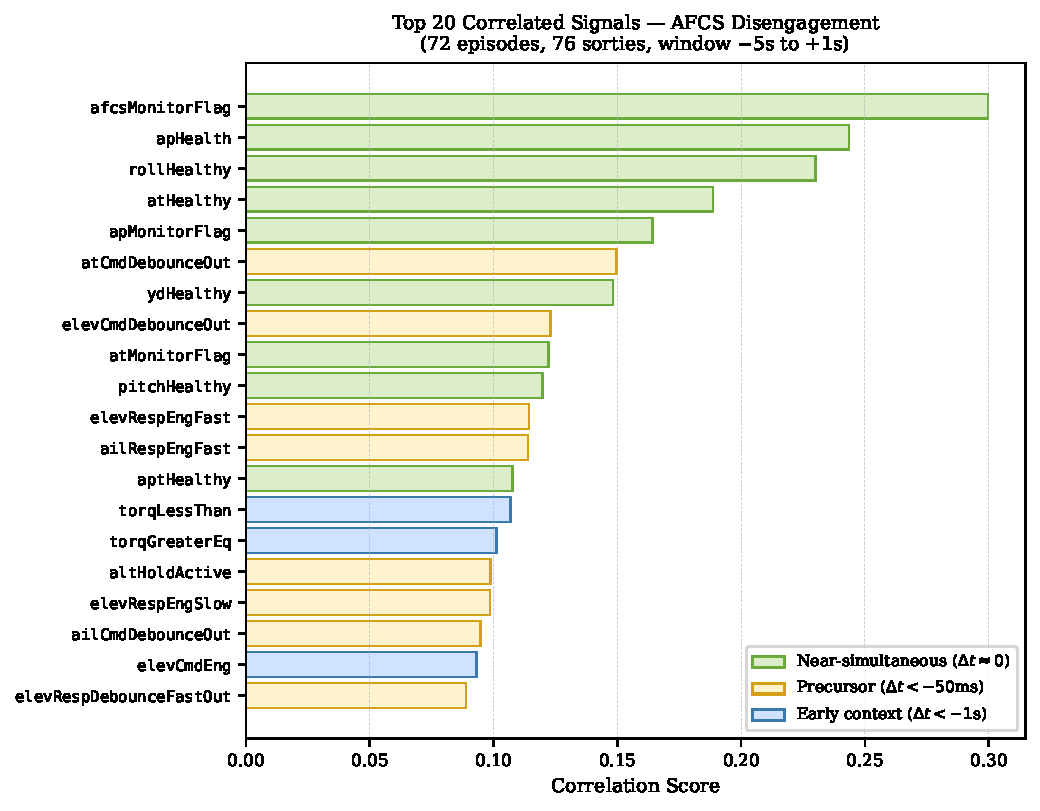
\includegraphics[width=\textwidth]{plots/plot_correlations.pdf}
  \caption{Top 20 correlated signals ranked by score. Colours indicate temporal
    cluster: green = near-simultaneous with fault trigger, yellow = precursor
    ($\Delta t < -50$\,ms), blue = early contextual ($\Delta t < -1$\,s).}
  \label{fig:correlations}
\end{figure}

\begin{figure}[htbp]
  \centering
  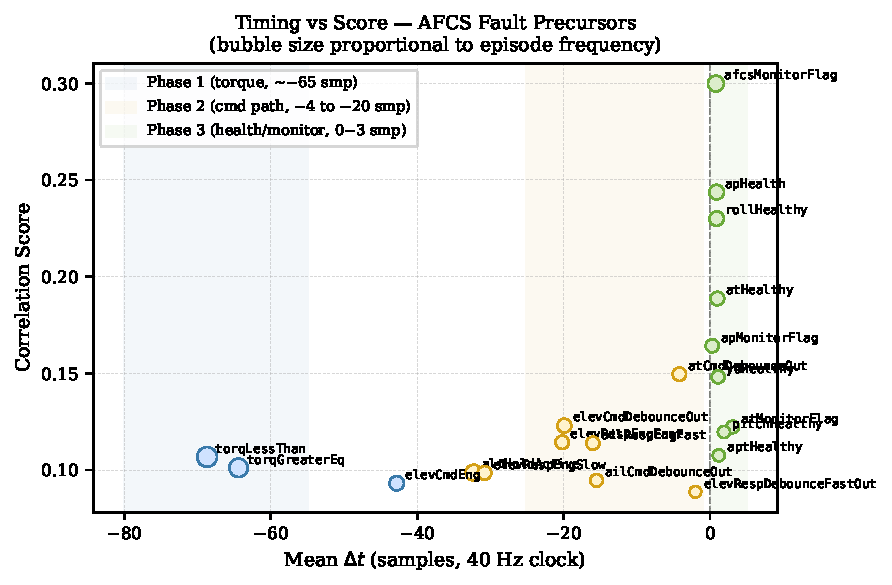
\includegraphics[width=0.9\textwidth]{plots/plot_timing.pdf}
  \caption{Correlation score vs mean timing offset (samples at 40\,Hz).
    Bubble size is proportional to episode frequency. The three shaded bands
    correspond to the Phase~1 (torque context), Phase~2 (command path), and
    Phase~3 (health/monitor) clusters described in Section~4.}
  \label{fig:timing}
\end{figure}

\begin{figure}[htbp]
  \centering
  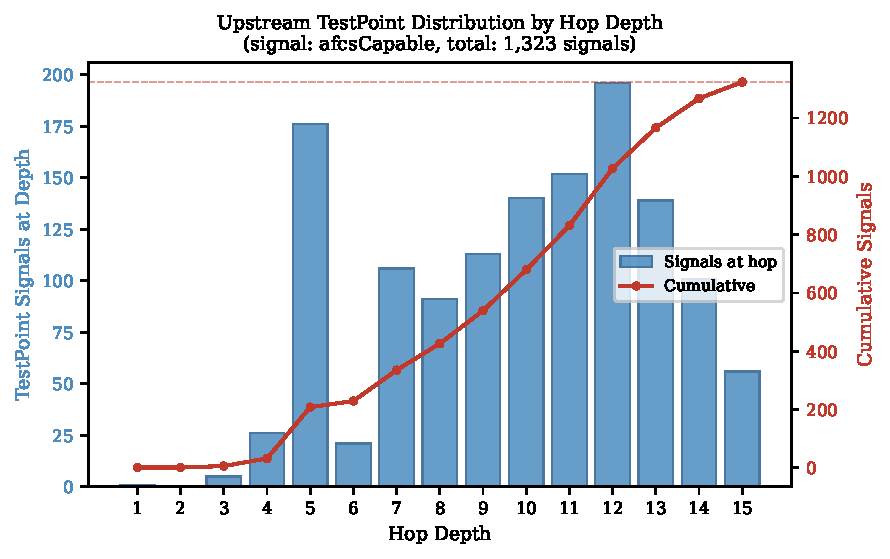
\includegraphics[width=0.85\textwidth]{plots/plot_hop_dist.pdf}
  \caption{Distribution of the 1{,}323 upstream TestPoint signals by BFS hop
    depth from \texttt{afcsCapable}. The cumulative curve shows that the
    majority of reachable signals are discovered within the first 8 hops;
    the depth-15 cap captures the full dependency cone.}
  \label{fig:hopdist}
\end{figure}

\begin{figure}[htbp]
  \centering
  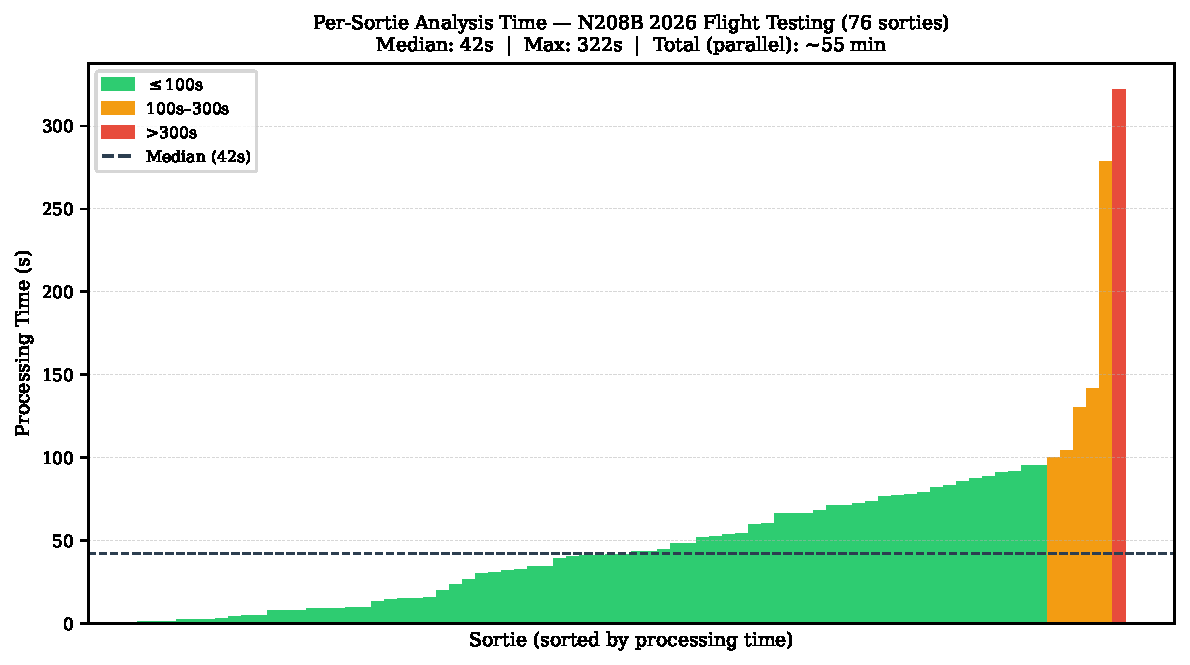
\includegraphics[width=\textwidth]{plots/plot_sortie_times.pdf}
  \caption{Per-sortie analysis JSON generation times across the 208B 2026
    flight testing dataset (76 sorties, sorted by duration). The majority
    complete in under 100\,s; the longest sorties ($>300$\,s) correspond to
    high-episode flights with dense signal transition data.}
  \label{fig:sortietimes}
\end{figure}

\clearpage
\section{Episode Classification Distribution}
\label{app:fault-dist}

Figure~\ref{fig:faultdist} shows the breakdown of all 72 AFCS disengagement
episodes by fault category, as classified by the same rule-based logic used
in the interactive HTML viewer. Categories are determined by examining boolean
signal transitions in the $\pm50$\,ms window around each episode trigger.

\begin{figure}[htbp]
  \centering
  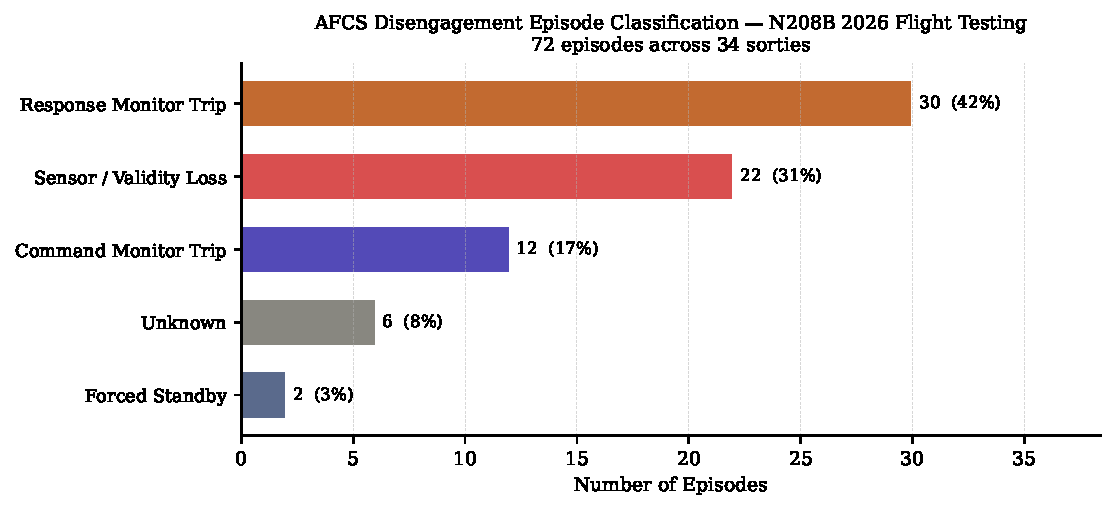
\includegraphics[width=\textwidth]{plots/plot_fault_dist.pdf}
  \caption{Distribution of AFCS disengagement episode types across 72 episodes
    (208B 2026 flight testing). Classification follows the rule-based
    \texttt{classifyExit()} logic in the HTML viewer: response and command
    monitor trips are identified by \texttt{*RespEng} and \texttt{*CmdEng}
    gate deactivations; sensor/validity loss by \texttt{*valid} or
    \texttt{*healthy} falling pre-trigger; unknown episodes have no
    classifiable boolean evidence in the trigger window.}
  \label{fig:faultdist}
\end{figure}

The 8\% unknown category represents episodes where no classifiable boolean
signal transition was observed in the trigger window --- either because the
causative signal was not captured as a TestPoint, the fault mechanism operates
below the classification rules' resolution, or the episode reflects a
multi-factor interaction not reducible to a single rule. These are the primary
candidates for deeper investigation via the upstream BFS trace and the Claude
API integration described in Section~\ref{sec:future}.

\clearpage
\section{Upstream BFS Trace Summary}
\label{app:upstream}

Table~\ref{tab:upstream} summarises the upstream BFS traversal from
\texttt{afcsCapable} using the trace graph from \repoTrace{}.

\begin{table}[h]
\centering
\caption{Upstream BFS traversal summary for \texttt{afcsCapable}.}
\label{tab:upstream}
\begin{tabular}{@{}lr@{}}
\toprule
\textbf{Parameter} & \textbf{Value} \\
\midrule
Target signal          & \texttt{afcsCapable} \\
Trace graph version    & \texttt{traceData-EOC-714-00001-05.01.02.json} \\
Graph size             & 22{,}361 nodes \quad 137{,}153 edges \\
Max hop depth          & 15 \\
Upstream TestPoints found & 1{,}323 \\
Correlated signals (in fleet data) & 5 \\
Traversal time         & $< 2$\,s \\
\midrule
\multicolumn{2}{@{}l}{\textit{Selected upstream signals with fleet correlation}} \\
\midrule
\texttt{afcsMonitorFlag} (hop~1) & score 0.300, freq 31.9\%, $\bar{\Delta t} = +0.8$\,samples \\
\texttt{apMonitorFlag} (hop~2)   & score 0.164, freq 16.7\%, $\bar{\Delta t} = +0.3$\,samples \\
\texttt{apHealth} (hop~3)        & score 0.244, freq 25.0\%, $\bar{\Delta t} = +0.9$\,samples \\
\texttt{rollHealthy} (hop~4)     & score 0.230, freq 23.6\%, $\bar{\Delta t} = +0.9$\,samples \\
\texttt{atHealthy} (hop~4)       & score 0.189, freq 19.4\%, $\bar{\Delta t} = +1.0$\,samples \\
\bottomrule
\end{tabular}
\end{table}

\clearpage
\section{HTML Viewer --- Fleet Summary}
\label{app:viewer}

The following figures are captured directly from the \repoFTA{} interactive
HTML viewer loaded with the full 208B 2026 flight testing dataset (76 sorties,
72 AFCS disengagement episodes). All classification, timing, and mode
attribution is computed client-side in the browser with no server dependency.

\begin{figure}[htbp]
  \centering
  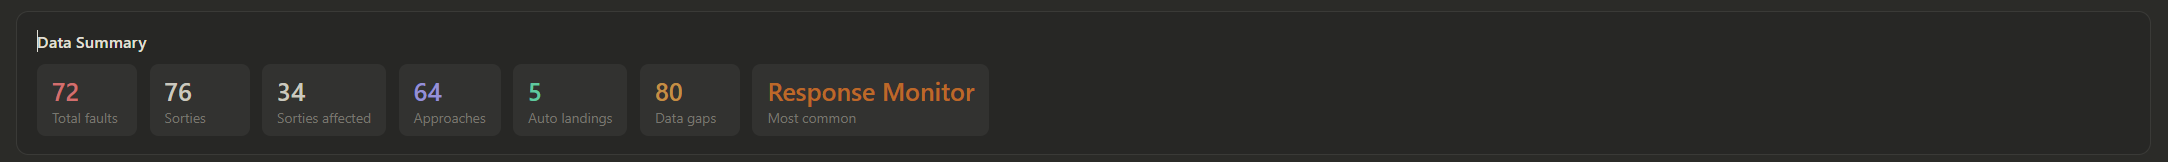
\includegraphics[width=\textwidth]{plots/html_data_summary.png}
  \caption{Fleet-level data summary header. The dataset spans 76 sorties with
    72 total AFCS fault events across 34 affected sorties (45\% fleet
    exposure), 64 captured approaches, and 5 automatic landings. The 80 data
    gap flags indicate recording dropouts that may conceal additional fault
    events, underscoring the importance of gap-aware analysis. Response Monitor
    is the most prevalent fault category fleet-wide.}
  \label{fig:html-summary}
\end{figure}

\begin{figure}[htbp]
  \centering
  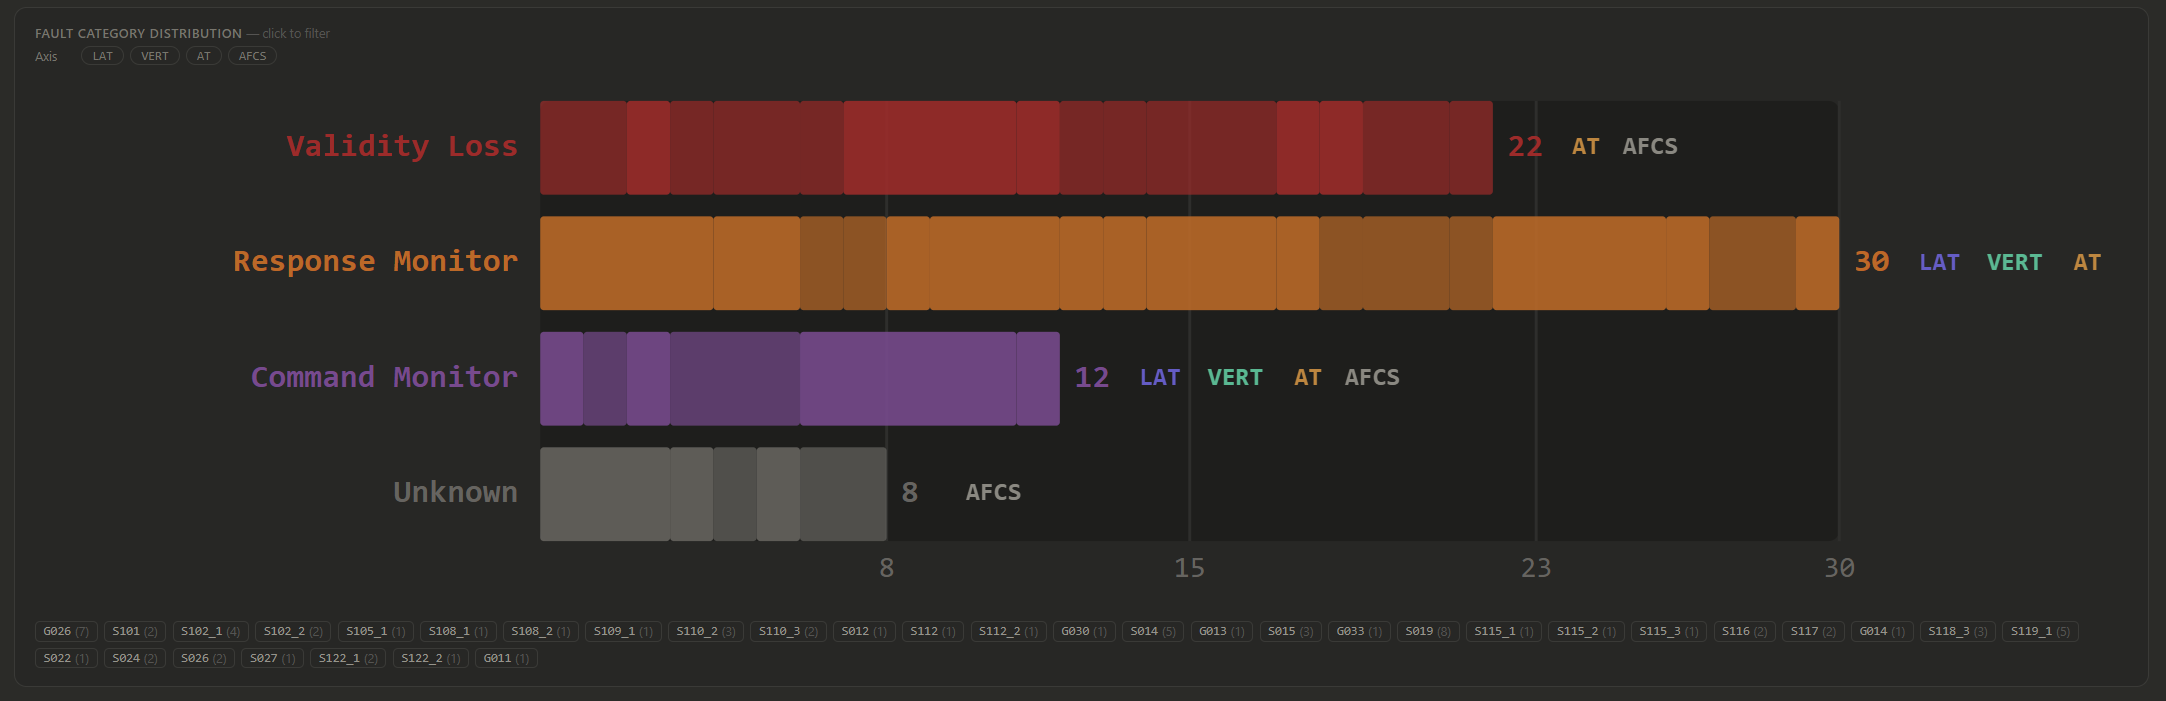
\includegraphics[width=\textwidth]{plots/html_fault_distribution.png}
  \caption{Fault category distribution across all 72 episodes. Response Monitor
    trips (30 events, 42\%) dominate, occurring across all three primary
    control axes (LAT, VERT, AT), indicating a systemic sensitivity in the
    monitor thresholds rather than an isolated axis failure. Validity Loss (22
    events, 31\%) is predominantly autothrottle-axis, consistent with the
    torque exceedance data presented in Figure~\ref{fig:html-torque}. Command
    Monitor trips (12 events, 17\%) are distributed across all axes. The 8
    Unknown events (11\%) are restricted to the AFCS-level and represent
    the highest-priority investigation targets, as their causative signals
    were not observable in the captured TestPoint set.}
  \label{fig:html-faultdist}
\end{figure}

\begin{figure}[htbp]
  \centering
  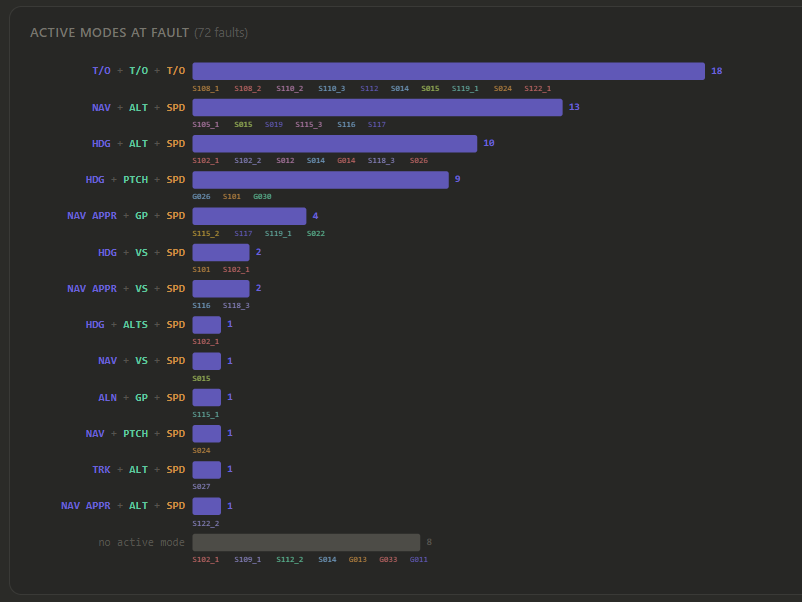
\includegraphics[width=\textwidth]{plots/html_active_modes.png}
  \caption{Active AFCS mode combination at the time of each fault event (72
    faults). Takeoff configuration (T/O\,+\,T/O\,+\,T/O) accounts for the
    single largest fault cohort with 18 events (25\% of all faults), suggesting
    that the takeoff phase presents elevated monitor sensitivity relative to
    other flight phases --- likely driven by high torque transients during
    initial climb. The next two cohorts (NAV\,+\,ALT\,+\,SPD at 13 events and
    HDG\,+\,ALT\,+\,SPD at 10 events) represent cruise-phase disengagements.
    The 8 faults with no recorded active mode correspond to episodes where mode
    state data was unavailable, not to standby-mode operation.}
  \label{fig:html-modes}
\end{figure}

\begin{figure}[htbp]
  \centering
  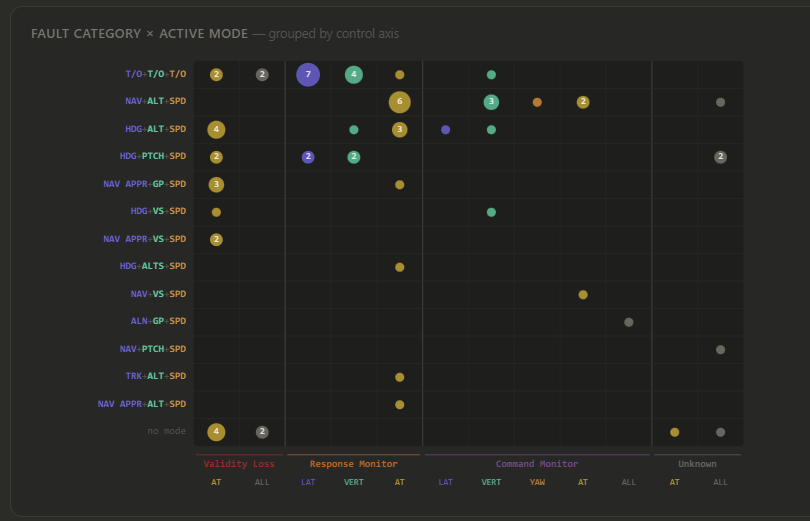
\includegraphics[width=\textwidth]{plots/html_fault_mode_matrix.png}
  \caption{Cross-tabulation of fault category, active mode, and control axis
    (bubble matrix). Bubble area is proportional to event count; category colour
    matches the distribution chart. The concentration of Response Monitor
    events in the takeoff row across all three axes (LAT, VERT, AT)
    distinguishes takeoff from cruise-phase disengagements, where Command
    Monitor trips become more prevalent on the lateral and vertical axes.
    The no-mode row is dominated by Validity Loss on the AT axis,
    consistent with episodes where autothrottle validity degraded before a
    stable mode was established. This view directly guides corrective action:
    reducing takeoff Response Monitor sensitivity and investigating AT validity
    sources are the two highest-leverage interventions.}
  \label{fig:html-matrix}
\end{figure}

\begin{figure}[htbp]
  \centering
  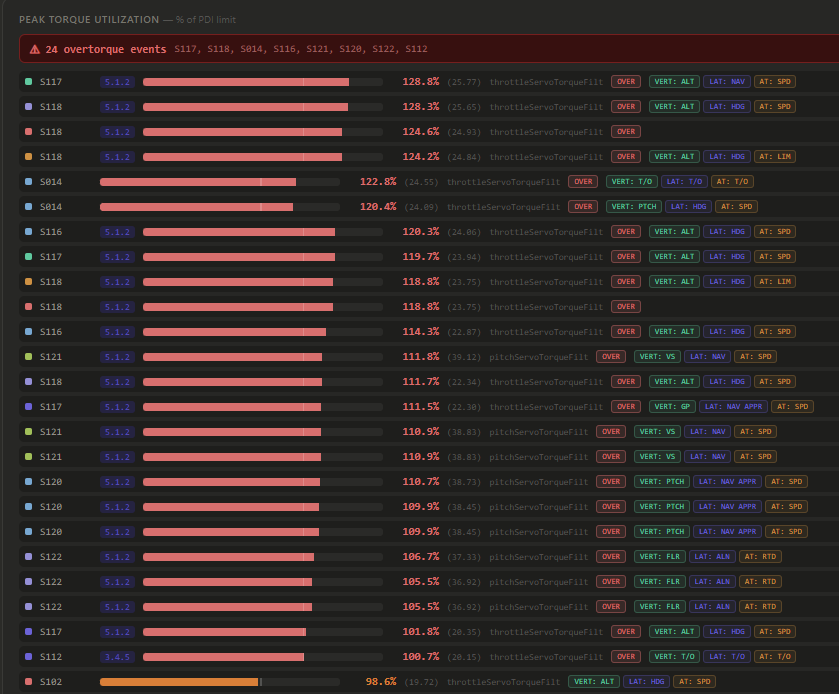
\includegraphics[width=\textwidth]{plots/html_peak_torque.png}
  \caption{Peak servo torque utilisation as a percentage of PDI limit, sorted
    descending. 24 overtorque events were detected across 8 sorties
    (S117, S118, S014, S116, S121, S120, S122, S112), with peak utilisation
    reaching 128.8\% of limit. The majority of overtorque events involve
    \texttt{throttleServoTorqueFilt} (autothrottle axis) during
    ALT\,+\,HDG\,+\,SPD and ALT\,+\,NAV\,+\,SPD modes, directly linking
    torque exceedances to the AT-axis Validity Loss faults seen in
    Figure~\ref{fig:html-faultdist}. The \texttt{pitchServoTorqueFilt}
    overtorques on S121 occur in VS\,+\,NAV\,+\,SPD mode, a distinct cluster
    warranting separate investigation. This automated detection removes the
    need for manual post-sortie torque review across 76 sorties.}
  \label{fig:html-torque}
\end{figure}

\begin{figure}[htbp]
  \centering
  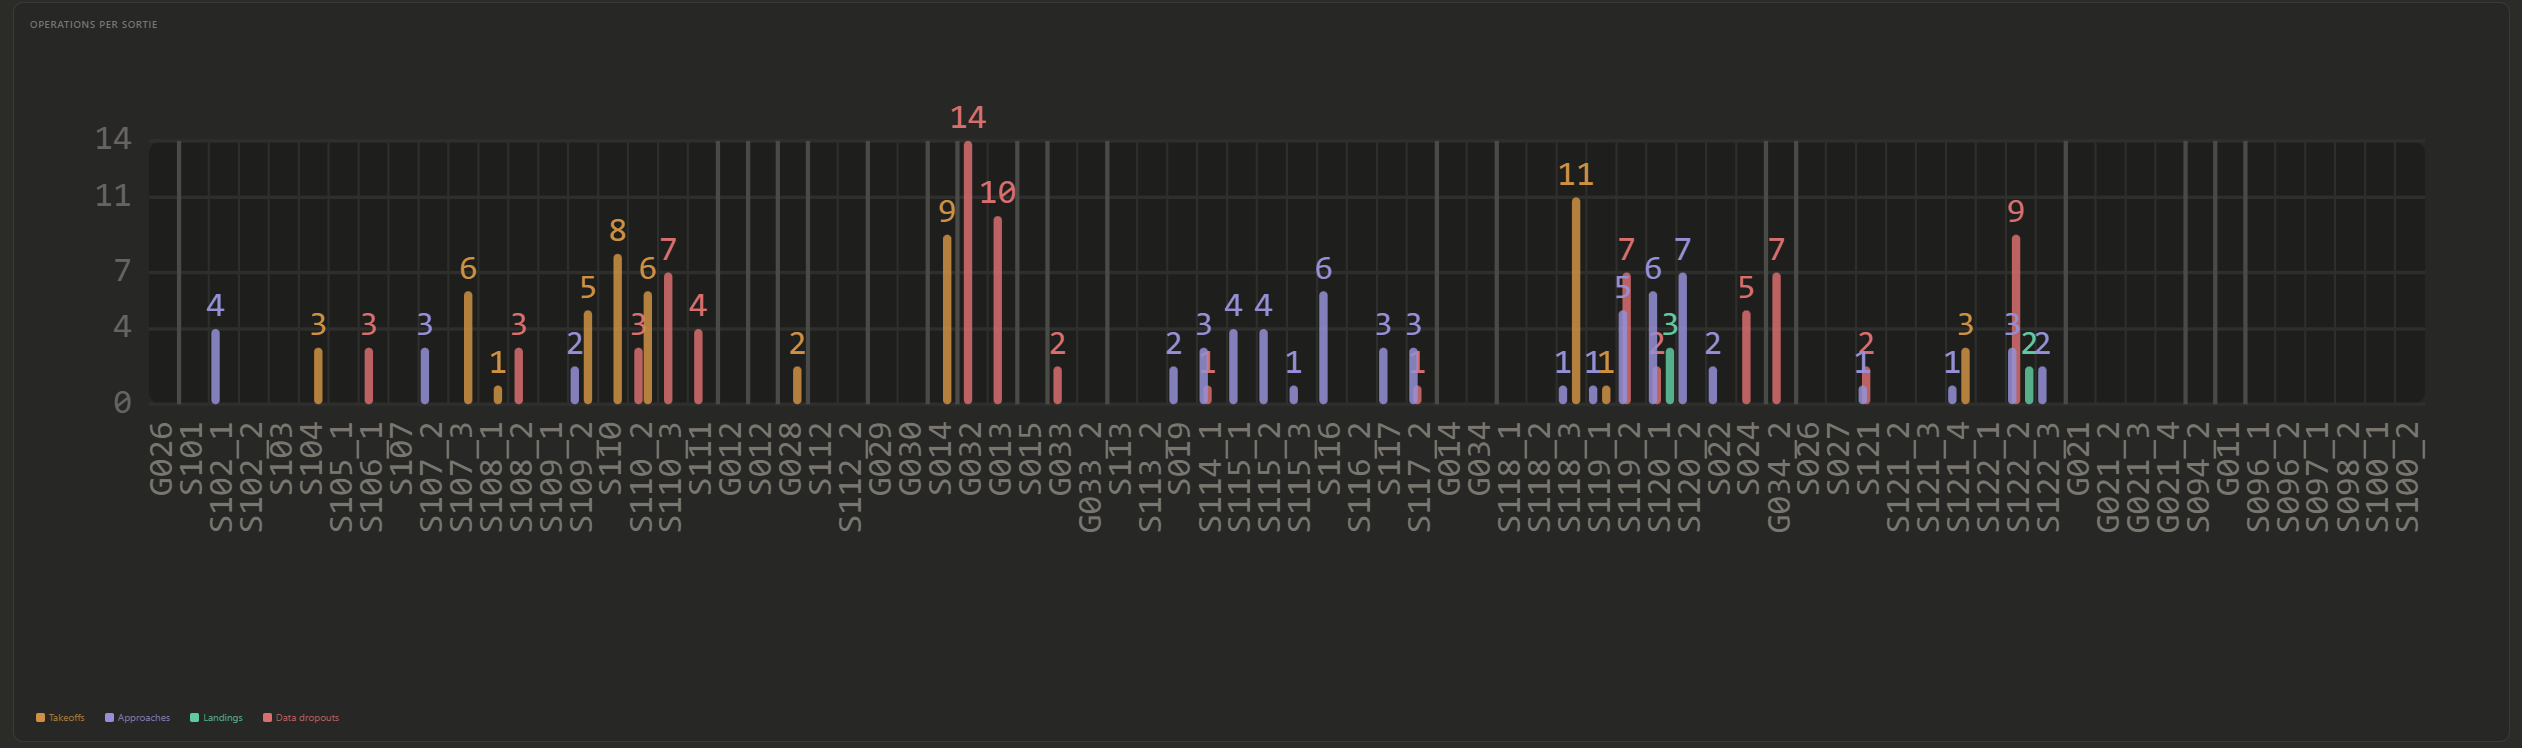
\includegraphics[width=\textwidth]{plots/html_ops_per_sortie.png}
  \caption{Operations per sortie (takeoffs, approaches, landings, and data
    dropouts) across all 76 sorties. Operational tempo varies significantly:
    sorties G030--G032 executed up to 14 operations per flight. The data
    dropout count (red) highlights that recording gaps are widespread rather
    than isolated; several sorties show more dropouts than approaches,
    suggesting the data gap detection mechanism is identifying genuine
    interruptions in the IADS recording stream that would otherwise silently
    bias fault statistics.}
  \label{fig:html-ops}
\end{figure}

\end{appendices}

\end{document}
